\localauthor{
	\begin{itemize}
		\item RSA: Sebastian Vogt
		\item Control Schicht: Sebastian Vogt
		\item Business Schicht: Johannes Garstenauer
		\item Persistence Schicht: Sebastian Vogt
		\item Cross-Cutting Concerns: Sebastian Vogt
	\end{itemize}
}

\newcommand{\classtable}[1]{\begin{longtable}[H]{m{5cm}m{9cm}}
                                \hline
                                \textbf{Klassenname} & \textbf{Beschreibung} \\
                                \hline
                                \hline
                                #1
\end{longtable}
}

\newcommand{\classentry}[2]{\textbf{#1} & #2 \\
	\hline
}

\subsection{Klassendiagramm}

Im folgenden Klassendiagramm wurden folgende Konventionen verwendet:
\begin{itemize}
    \item Properties sind als private Attribute modelliert.
    Konstruktoren sind ausgespart.
    \item Referenzattribute auf andere Klassen des Diagramms sind als Pfeile dargestellt.
    Diese haben standardmäßig keine Getter und Setter, außer anders angegeben.
    \item Gestrichelte Pfeile sind \emph{use-Pfeile}, egal ob diese mit \emph{<<use>>} versehen sind oder nicht.
\end{itemize}

Weitere Informationen zur Interpretation des Diagramms finden sich in den jeweiligen Packages.

\begin{figure}[H]
	\centering
	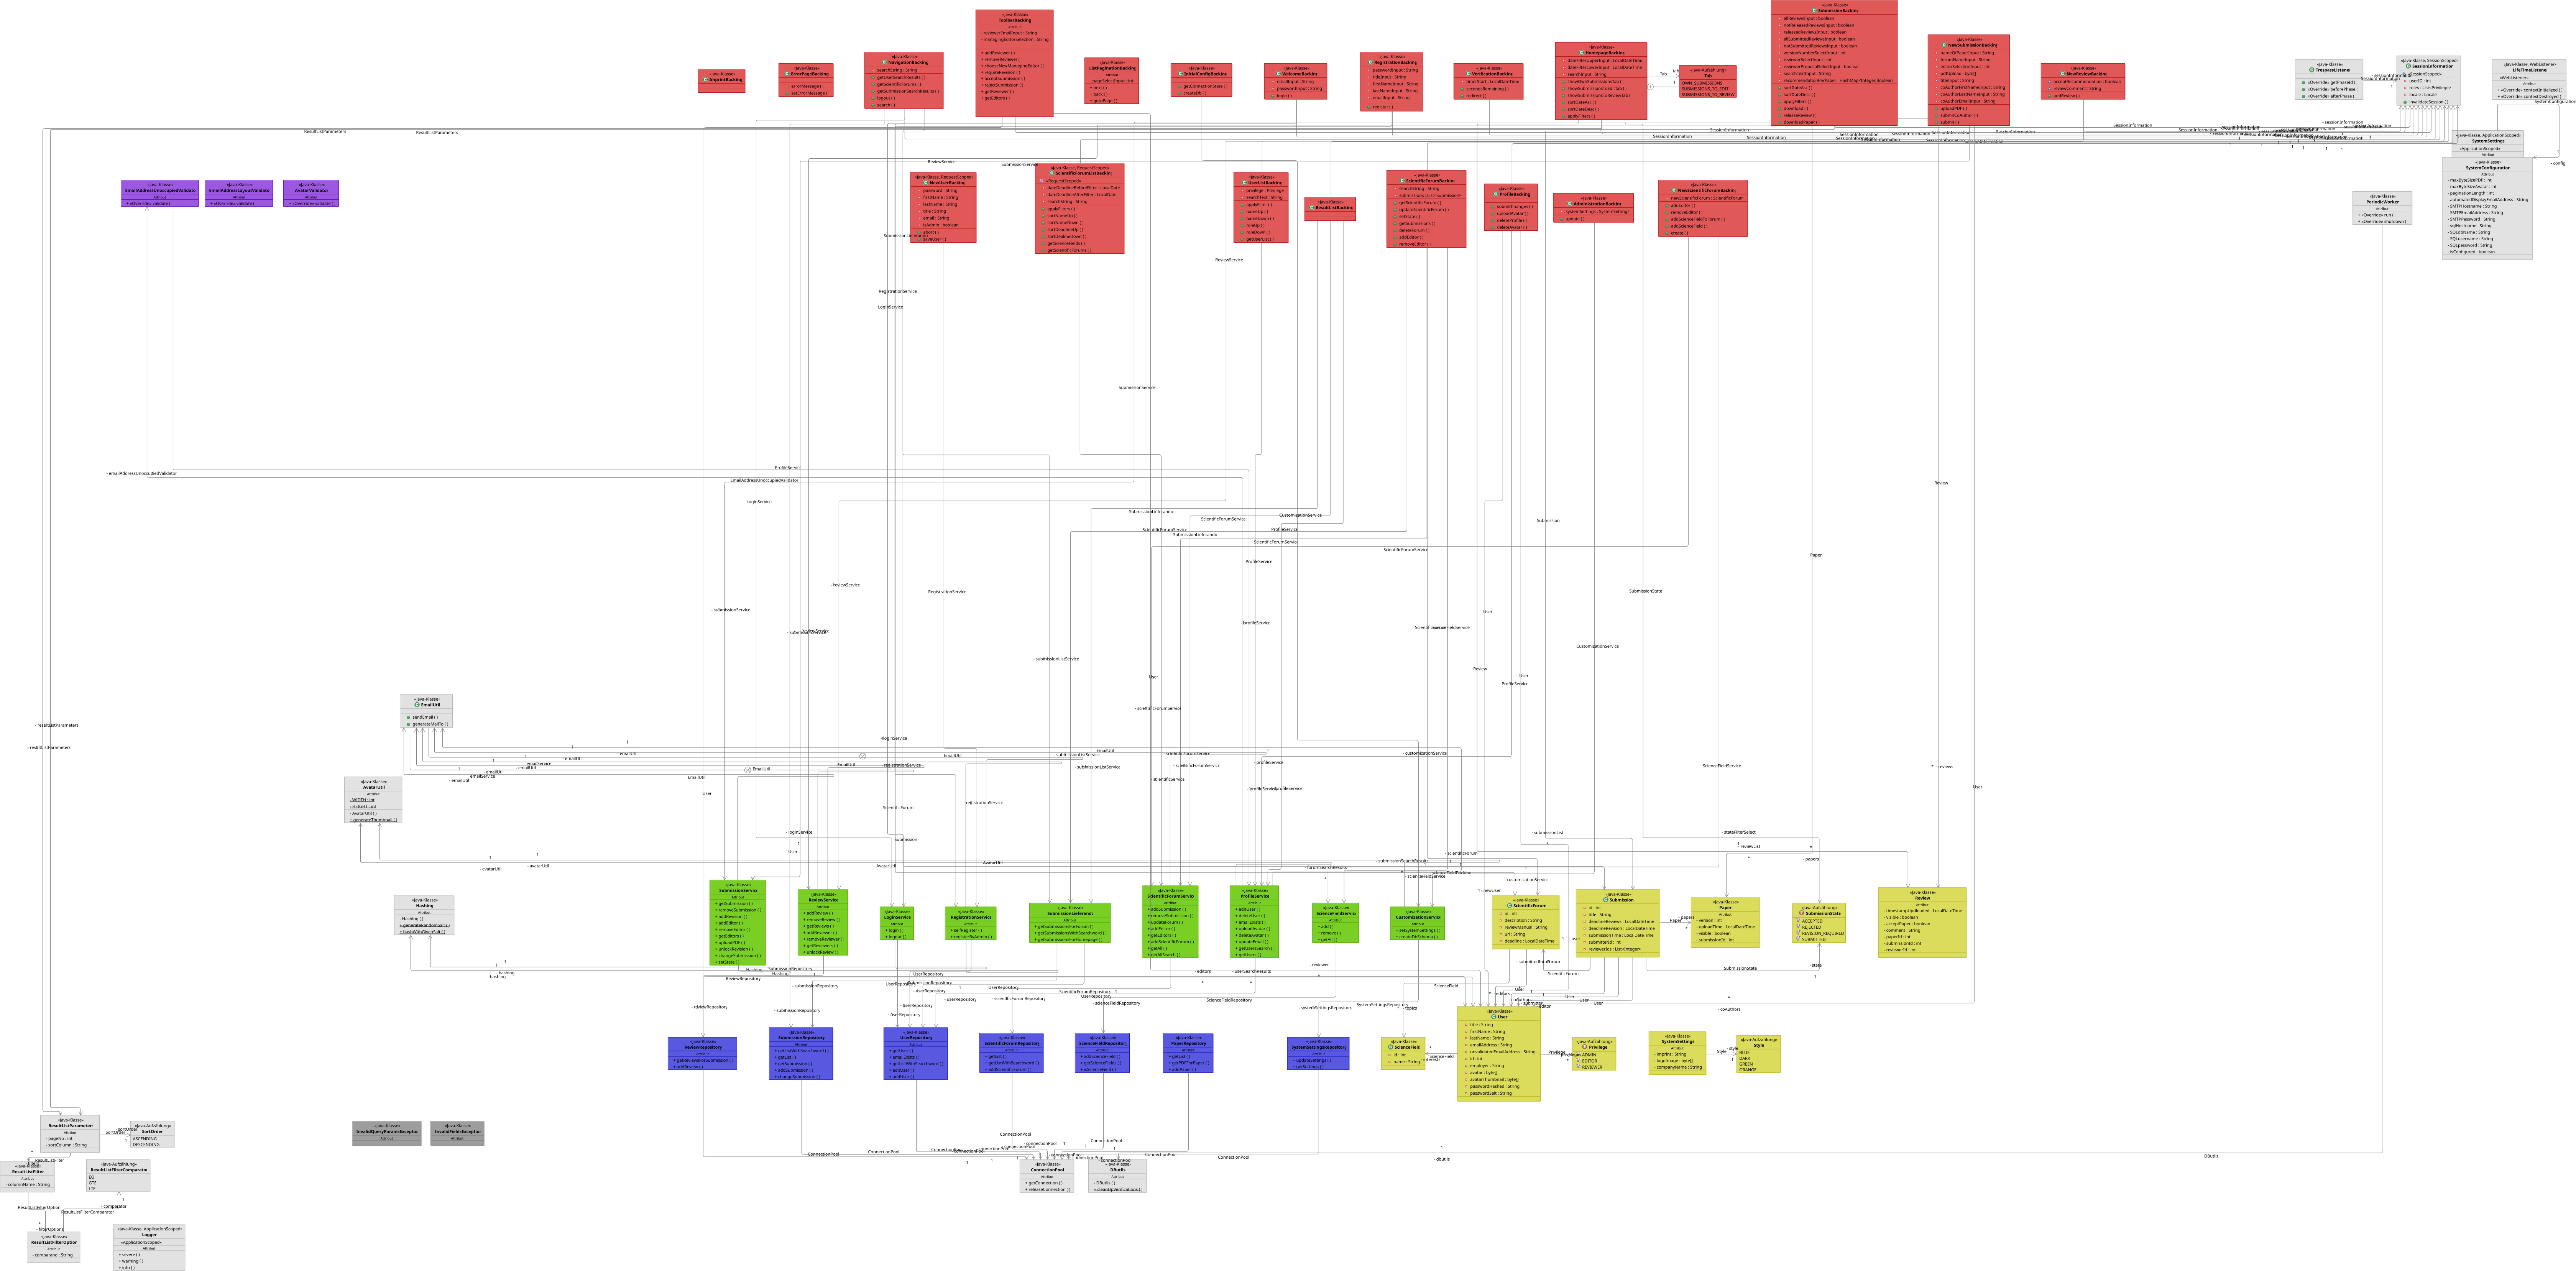
\includegraphics[width=\linewidth]{graphics/klassendiagramm_png}
\end{figure}

% Hier Klassendiagramm mal irgendwann einfügen.

\subsection{Klassenbeschreibungen}

\subsubsection{de.lases.global.logging}

\begin{figure}[H]
	\centering
	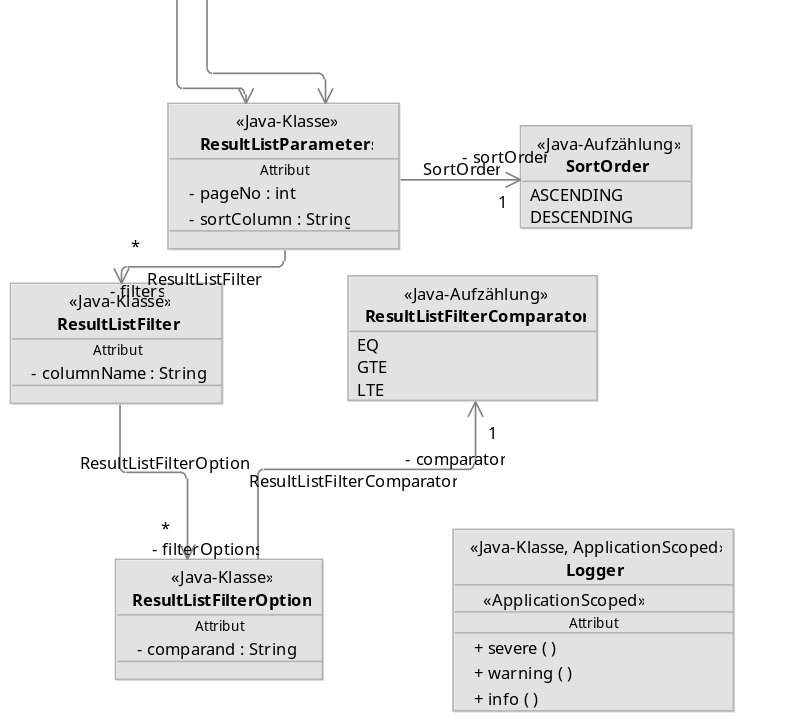
\includegraphics[height=3cm]{graphics/global_util}
\end{figure}

\classtable{
	\classentry{Logging}{This Logger allows logging in different log-levels.}
}

\subsubsection{de.lases.global.transport}

Im folgenden Diagramm gilt für die Klassen mit dickem schwarzem Rand folgende Konvention:
\begin{itemize}
	\item Die Zuordnungen zwischen den Klassen werden nicht durch Java Zeiger realisiert, sondern durch Speichern der Id des jeweiligen Objekts.
	\item Bei einer $x \rightarrow 1$ Beziehung (mit $x \in \{1, *\}$) merkt sich das Objekt auf der Linken Seite die Id des zugeordneten Objektes
	\item Bei einer $x \rightarrow *$ Beziehung merkt sich das Objekt auf der Linken Seite \emph{keine} Liste der zugehörigen Ids. Zuordnungen sind in diese Richtung also nicht unmittelbar traversierbar.
\end{itemize}
Die Vollständigkeit der DTOs wurde gegen das ER-Diagramm gegengeprüft.
natürlich gibt es aber auch DTOs, die nicht direkt aus dem ER-Diagramm kommen.
\begin{figure}[H]
	\centering
	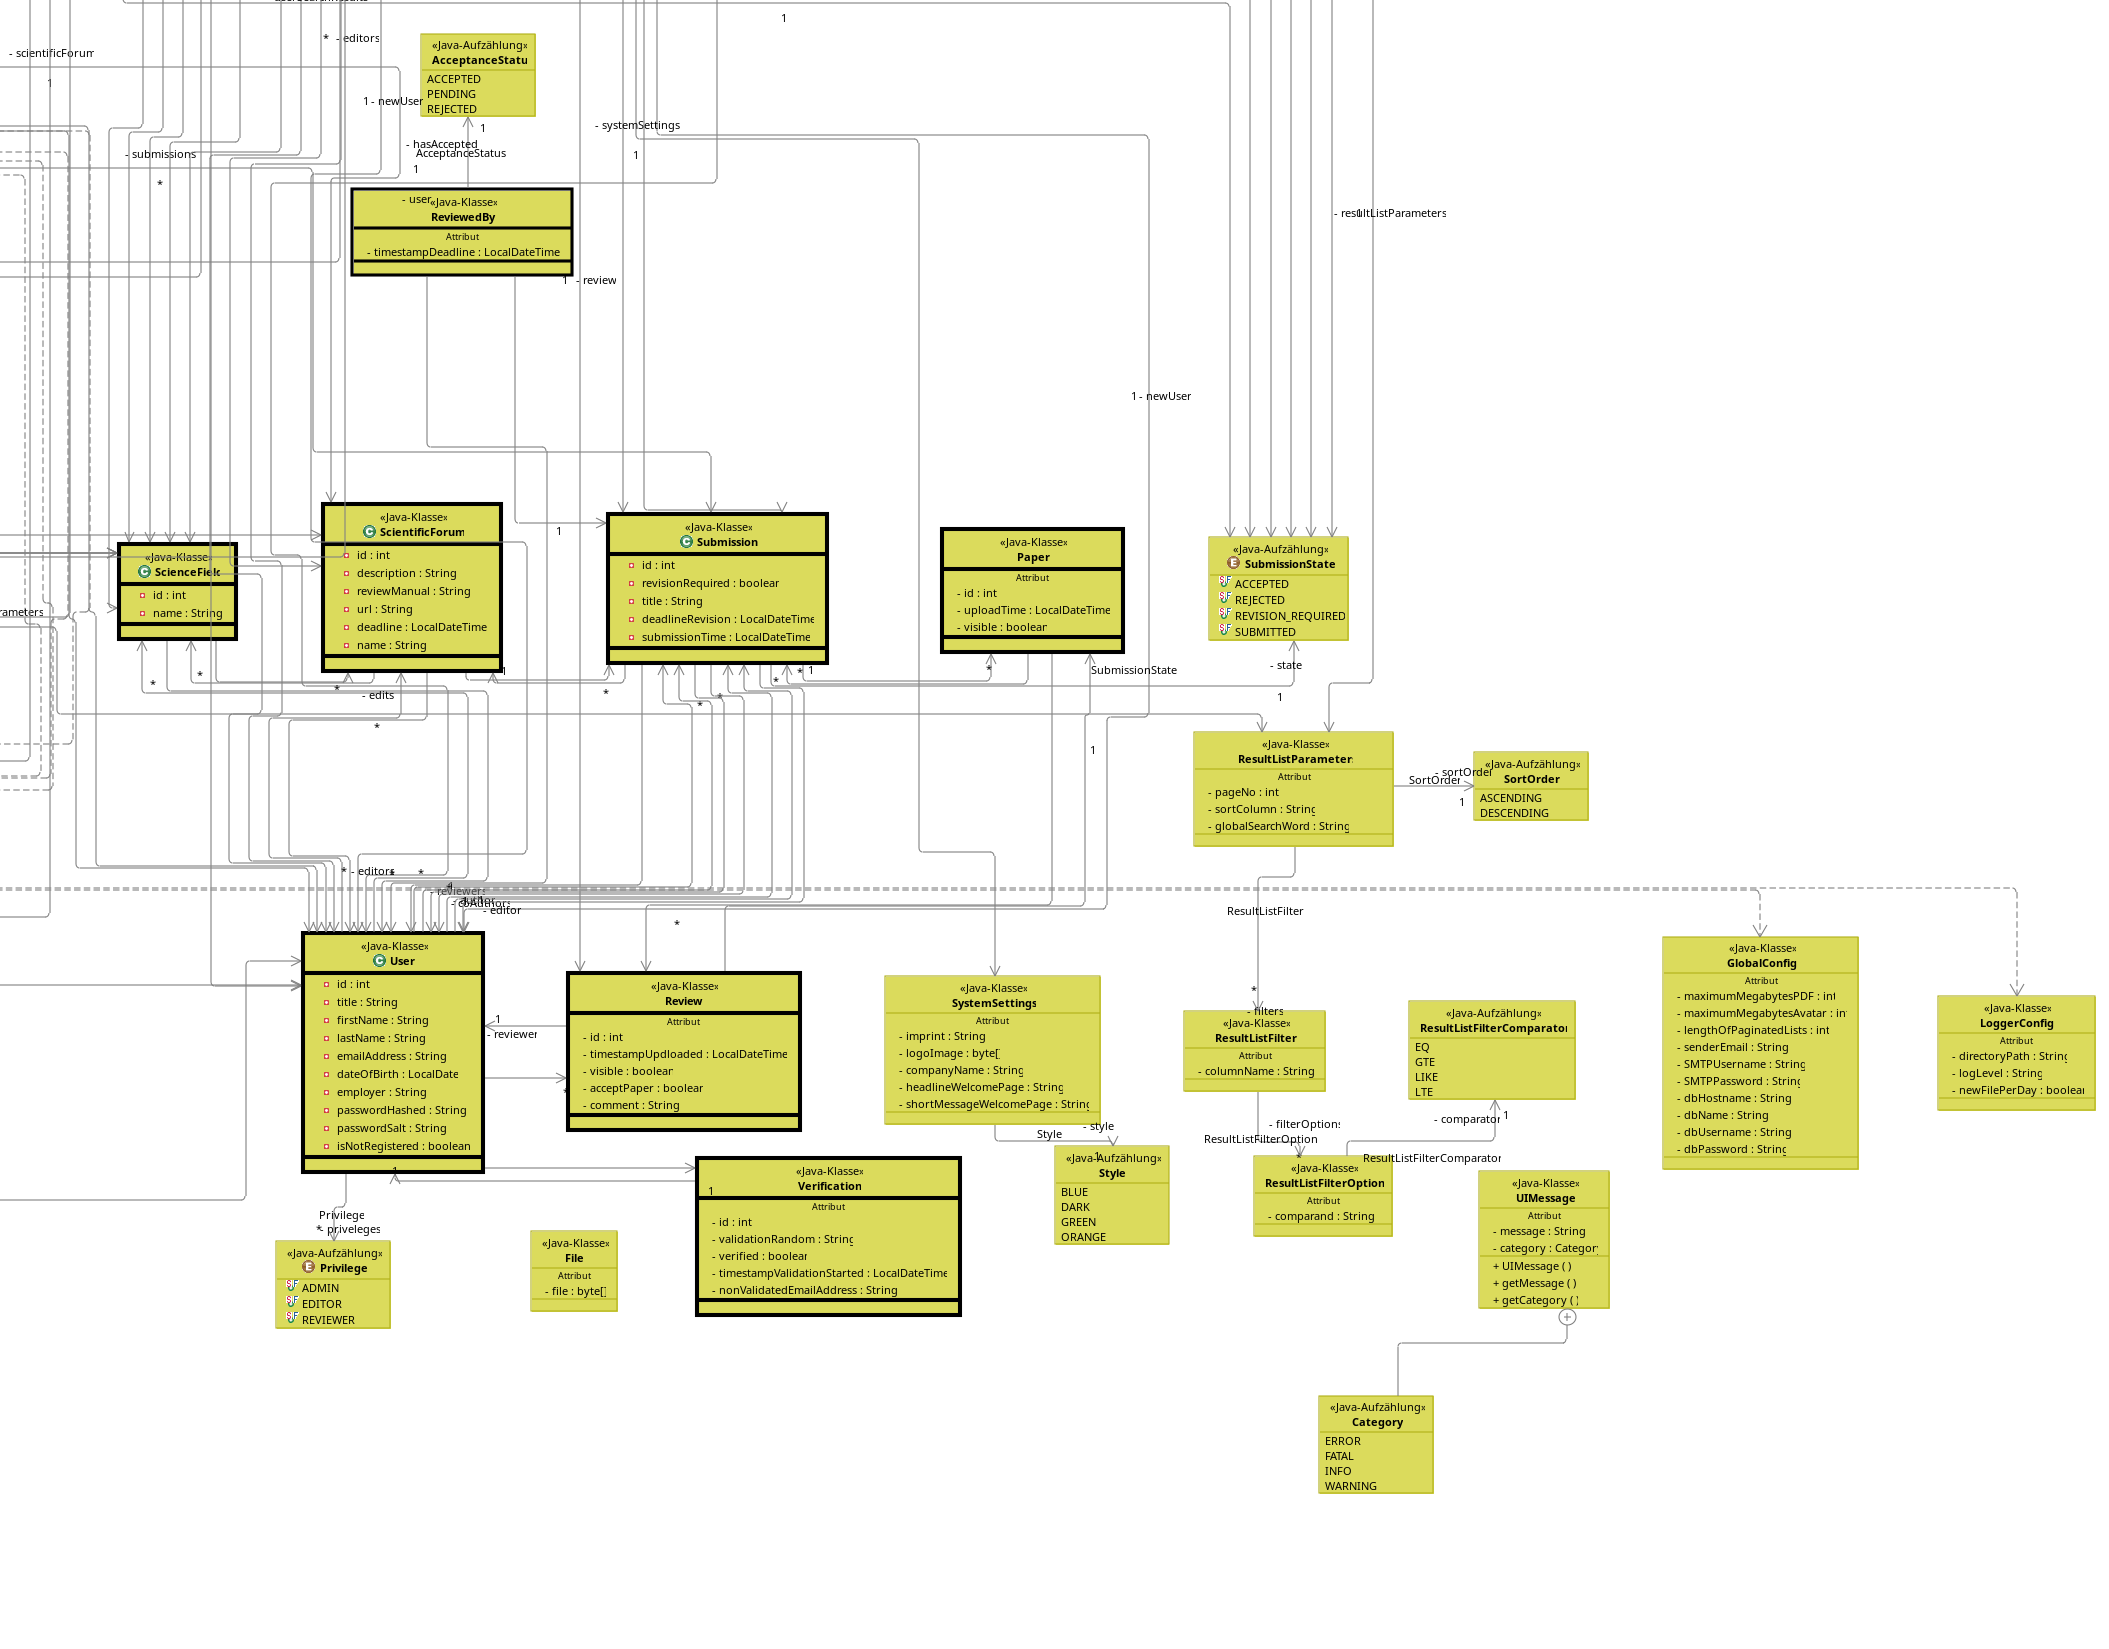
\includegraphics[height=3cm]{graphics/global_transport}
\end{figure}

\classtable{
	\classentry{Paper}{This DTO represents a paper.}
	\classentry{Privilege}{This represents a user privilege.}
	\classentry{Review}{This DTO represents a review.}
	\classentry{ScienceField}{This DTO represents a field of Science.}
	\classentry{ScientificForum}{This DTO represents a forum}
	\classentry{Style}{This represents a user interface style.}
	\classentry{Submission}{This DTO represents a submission.}
	\classentry{SubmissionState}{This represents a submissions state.}
	\classentry{SystemSettings}{This DTO represents the system settings.}
	\classentry{User}{This DTO represents a user.}
	\classentry{ResultListParameters}{This class bundles parameters for requesting lists from the database. This includes page numner, sorting of the results and filtering of the results}
	\classentry{SortOrder}{A List can be sorted in ascending or descending order}
	\classentry{ResultListFilter}{A filter that can be applied on a column of a table}
	\classentry{ResultListFilterOption}{A single comparison that can be used to construct a ResultListFilter}
	\classentry{ResultListFilterComparator}{The three comparators equal to, less than or equal and greater than or equal}
	\classentry{GlobalConfig}{Holds all data that is read from the config file.}
	\classentry{Verification}{Bundles information about the verification process is somebody is newly registered or has just changed theirq email.}
	\classentry{File}{Encapsulates a file that is passed between the layers.}
	\classentry{ReviewedBy}{Stores Information about the relationship of a Submission and a User (the reviewer).}
	\classentry{AcceptanceStatus}{Holds the information wheather a requested reviewer has accepted or rejected the request or has yet to decide.}
}

\subsubsection{de.lases.control.backing}

Im Diagramm dieses Pakets sind folgende Punkte zu beachten:
\begin{itemize}
	\item Pfeile, die zur SessionInformation führen wurden aus Gründen der Übersichtlichkeit ausgespart und lediglich als Attribut dargestellt.
	Die SessionInformation hat natürlich trotzdem keine Getter und Setter.
	\item Alle backing Beans sind managed Beans.
\end{itemize}

\begin{figure}[H]
	\centering
	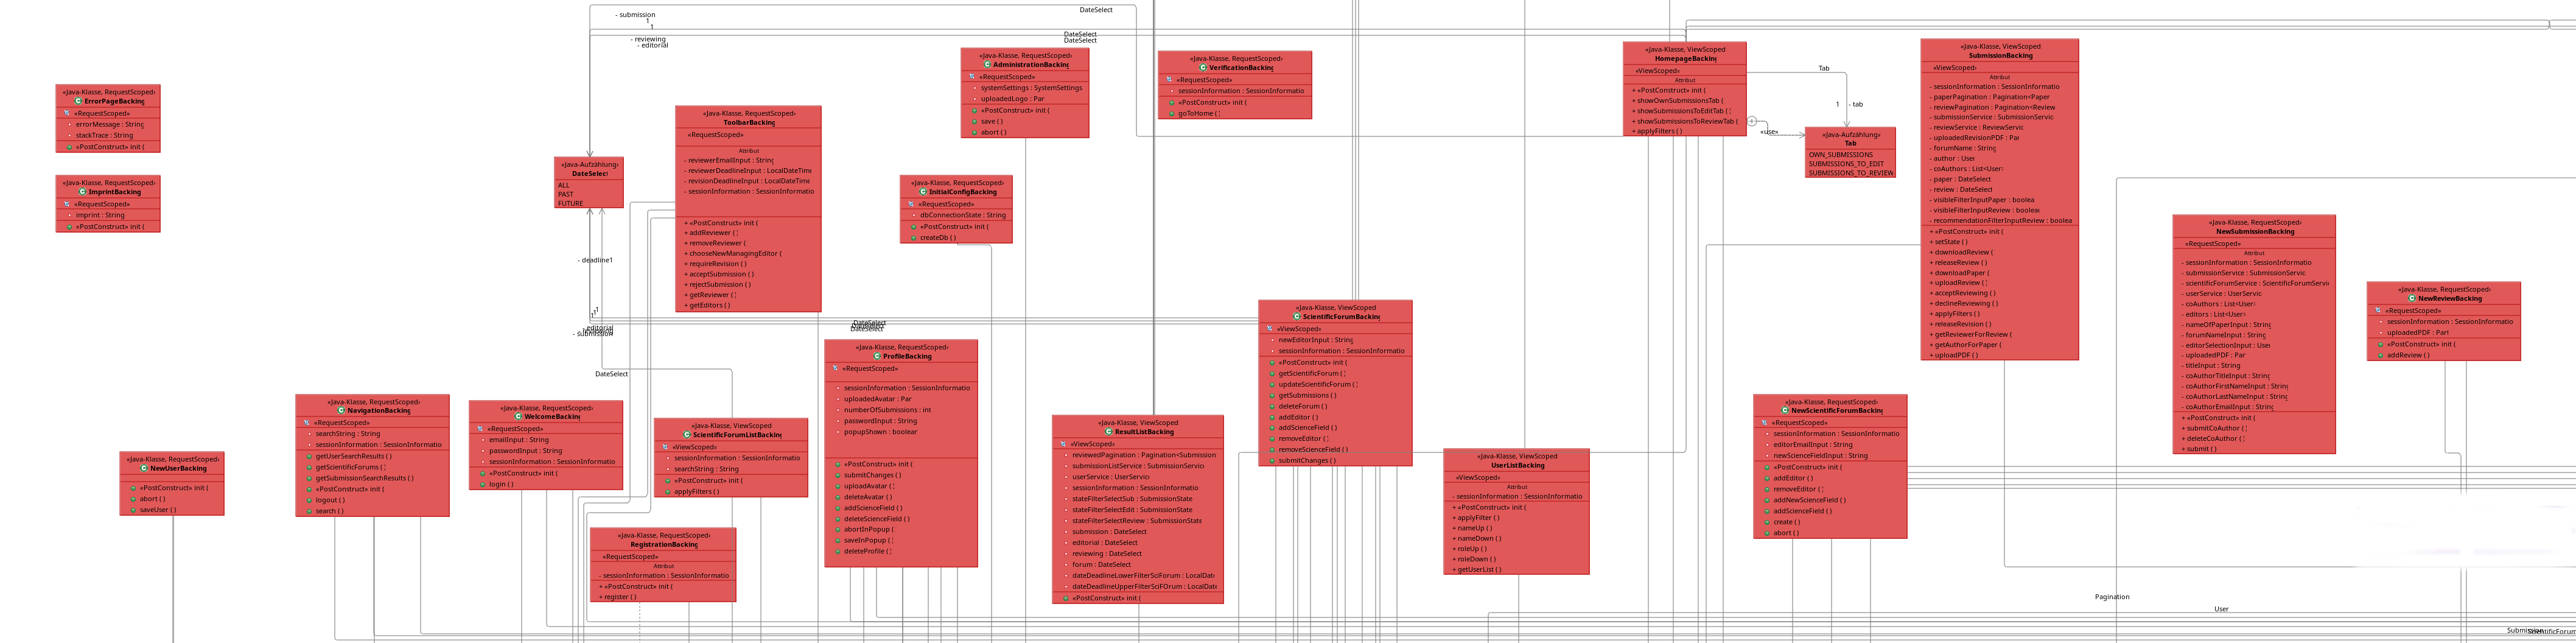
\includegraphics[width=0.9\linewidth]{graphics/control_backing}
\end{figure}

\classtable{
	\classentry{NewSubmissionBacking}{Backing bean for the page for creating a new submission.}
	\classentry{SubmissionBacking}{Backing bean for the submission page.}
	\classentry{NewReviewBacking}{Backing bean for the page for creating adding a new review.}
	\classentry{VerificationBacking}{Backing bean for the verification page.}
	\classentry{ToolbarBacking}{Backing bean for the side toolbar.}
	\classentry{NavigationBacking}{Backing bean for the navigation bar.}
	\classentry{WelcomeBacking}{Backing bean for the welcome and login page.}
	\classentry{RegistrationBacking}{Backing bean for the registration page.}
	\classentry{HomepageBacking}{Backing bean for the homepage for logged in users.}
	\classentry{NewUser}{Backing bean for the page for adding a new user.}
	\classentry{ScientificForumListBacking}{Backing bean for the list of scientific forums.}
	\classentry{UserListBacking}{Backing bean for the list of users.}
	\classentry{ResultListBacking}{Backing bean for the search result page.}
	\classentry{ScientificForumBacking}{Backing bean for the scientific forum page.}
	\classentry{NewScientificForumBacking}{Backing bean for the page for adding a new forum.}
	\classentry{ProfileBacking}{Backing bean for the profile page.}
	\classentry{AdministrationBacking}{Backing bean for the administration page.}
	\classentry{FooterBacking}{Backing bean for the footer template.}
}


\subsubsection{de.lases.control.internal}

\begin{figure}[H]
	\centering
	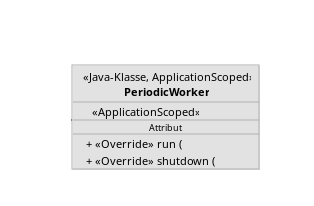
\includegraphics[height=3cm]{graphics/business_internal}
\end{figure}

\classtable{
	\classentry{TrespassListener}{Manages user access to resources, most importantly webpages.}
	\classentry{SessionInformation}{Wraps data saved in the session.}
	\classentry{LifeTimeListener}{Takes care of system start and shutdown operations}
	\classentry{ExceptionHandler}{Handles all Exceptions that leave the business layer by either showing a faces message or an error page.}
	\classentry{Pagination}{}
	\classentry{ImageServlet}{Serves avatars and logos.}
	\classentry{UIMessageGenerator}{}
	\classentry{UncheckedExceptionHandler}{arg2}
	\classentry{UncheckedExceptionHandlerFactory}{arg2}
}

\todo{erklaerung schreiben Pagination}

\subsubsection{de.lasses.control.validation}

\begin{figure}[H]
	\centering
	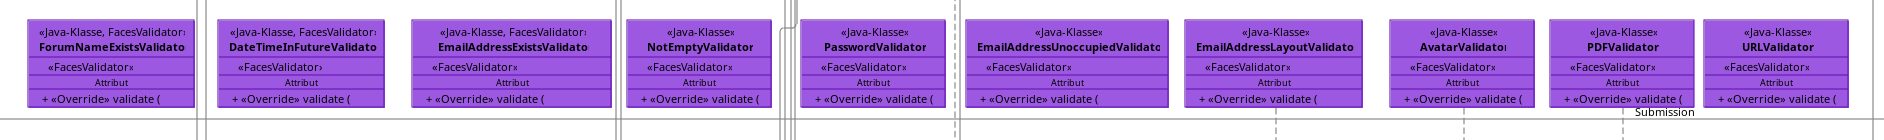
\includegraphics[height=3cm]{graphics/control_validation}
\end{figure}

\classtable{
    \classentry{AvatarValidation}{Validates that a suitable avatar image has been uploaded.}
    \classentry{PDFValidator}{Validates that a suitable PDF file has been uploaded.}
	\classentry{EmailAddressLayoutValidation}{Validates that a given String is a valid E-Mail Address.}
	\classentry{EmailAdressUnoccupiedValidator}{Validates that a given email is not already in use within the system.}
	\classentry{URLValidator}{Validates that a given String is a valid URL.}
	\classentry{PasswordValidator}{Checks if a password meets the minimum requirements for a password.}
	\classentry{NotEmptyValidator}{Checks if a free text imput is empty.}
	\classentry{EmailAddressExistsValidator}{Checks whether a given email address is a verified address in the system.}
	\classentry{DateTimeInFutureValidator}{Checks if a date input lies in the future.}
	\classentry{ForumNameExistsValidator}{Checks if a given input exists as a forum in the system.}
}

\subsubsection{de.lasses.control.util}

\begin{figure}[H]
	\centering
	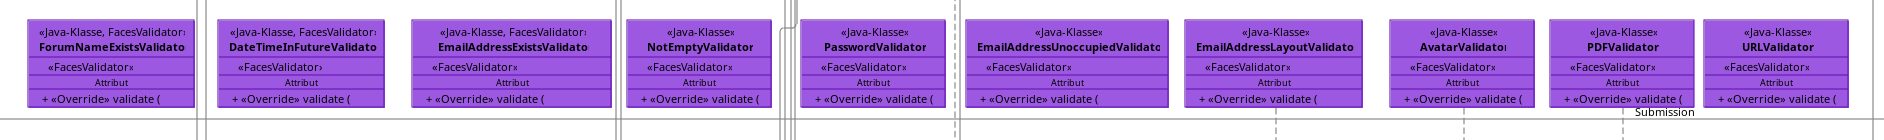
\includegraphics[height=3cm]{graphics/control_validation}
\end{figure}

\classtable{
	\classentry{URLGenerator}{Generates URLs with URL params.}

}

\subsubsection{de.lases.business.service}

\begin{figure}[H]
	\centering
	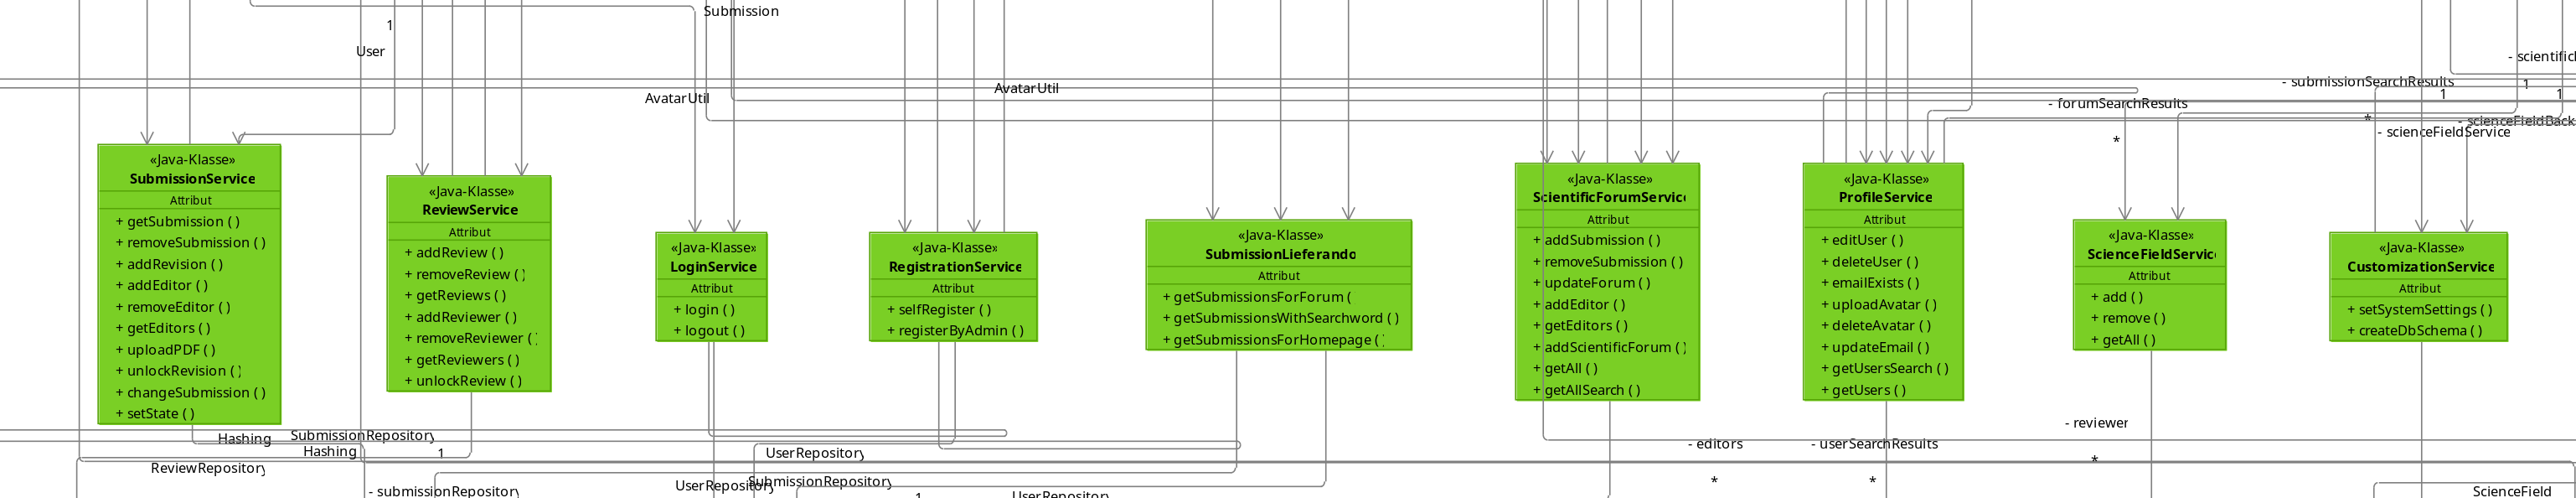
\includegraphics[width=0.9\linewidth]{graphics/business_service}
\end{figure}

\classtable{
	\classentry{CustomizationService}{Provides methods for the manipulation of system settings.}
	\classentry{ScienceFieldService}{Provides methods for adding and removing scientific categories.}
	\classentry{UserService}{Provides methods for the manipulation and removal of users.}
	\classentry{ScientificForumService}{Provides methods for the manipulation and creation of scientific forums.}
	\classentry{RegistrationService}{Provides methods for the creation of users.}
	\classentry{LoginService}{Provides methods for the login and logout operations.}
	\classentry{RevisionService}{Provides methods for the creation and manipulation of revisions for submissions.}
	\classentry{ReviewService}{Provides methods for the delivery, creation and removal of reviews.}
	\classentry{SubmissionService}{Provides methods for the delivery, creation, removal and manipulation of submissions.}
}

\subsubsection{de.lases.business.util}

\begin{figure}[H]
	\centering
	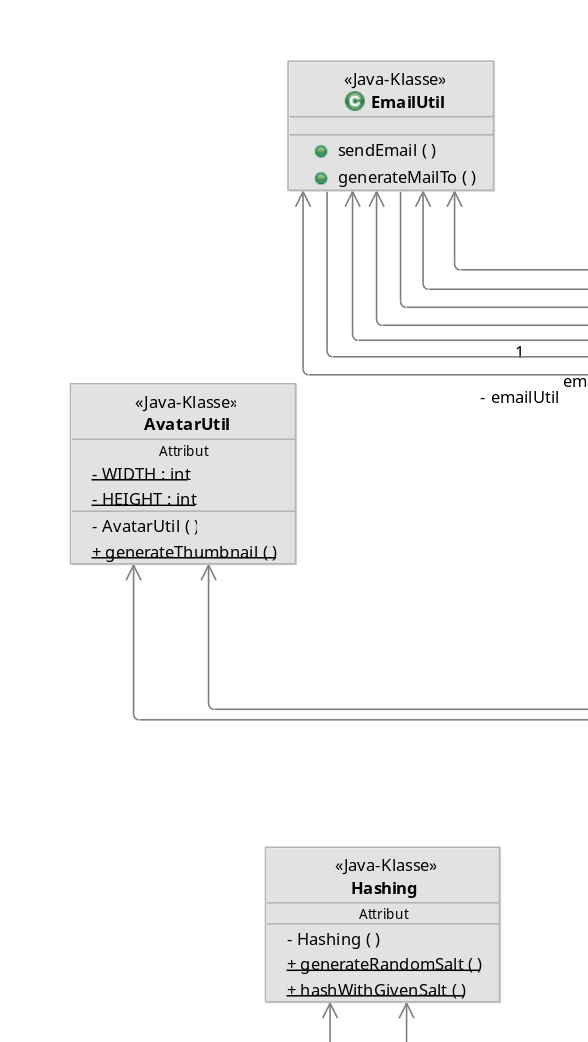
\includegraphics[height=3cm]{graphics/business_util}
\end{figure}

\classtable{
	\classentry{AvatarUtil}{Provides support in the generation of a thumbnail from an image.}
	\classentry{Hashing}{Provides support in the hashing of passwords.}
	\classentry{EmailUtil}{Provides support in the sending of emails, creation of \emph{mailto links} and checking of E-mail addresses.}
	\classentry{ConfigPropagator}{The purpose of this utility is to propagate the configuration data to the control layer.}
}

\subsubsection{de.lases.business.internal}

\begin{figure}[H]
	\centering
	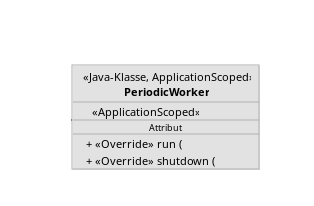
\includegraphics[height=3cm]{graphics/business_internal}
\end{figure}

\classtable{
	\classentry{PeriodicWorker}{Takes care of periodical database cleanup jobs.}
}

\subsubsection{de.lases.persistence.repository}

Im Folgenden Klassendiagramm gilt:
\begin{itemize}
	\item Jedes Repository ist für genau eine Entität im ER-Diagramm bzw. für genau ein DTO zuständig.
	\item Die Methode \emph{getList()} ist jeweils überladen. Falls man eine Liste von Objekten will, die mit einem bestimmten anderen Objekt \emph{a} direkt einer Relationship stehen (siehe ER-Diagramm), dann kann man \emph{a} an die Methode übergeben. Dies ist auch mit mehreren Relationships zugleich möglich.
	\item Spezifische \emph{addObject/removeObject} Methoden sind von der jeweils vorhandenen \emph{change} Methode insofern abzugrenzen, dass sie je Listen von zugeordneten Objekten bearbeiten. Die \emph{change} Methode kann nur Attribute mit Kardinalität 1 bearbeiten. Eine Ausnahme hierbei sind natürlich die \emph{get/set} Methoden für PDFs und Bilder.
\end{itemize}

\begin{figure}[H]
	\centering
	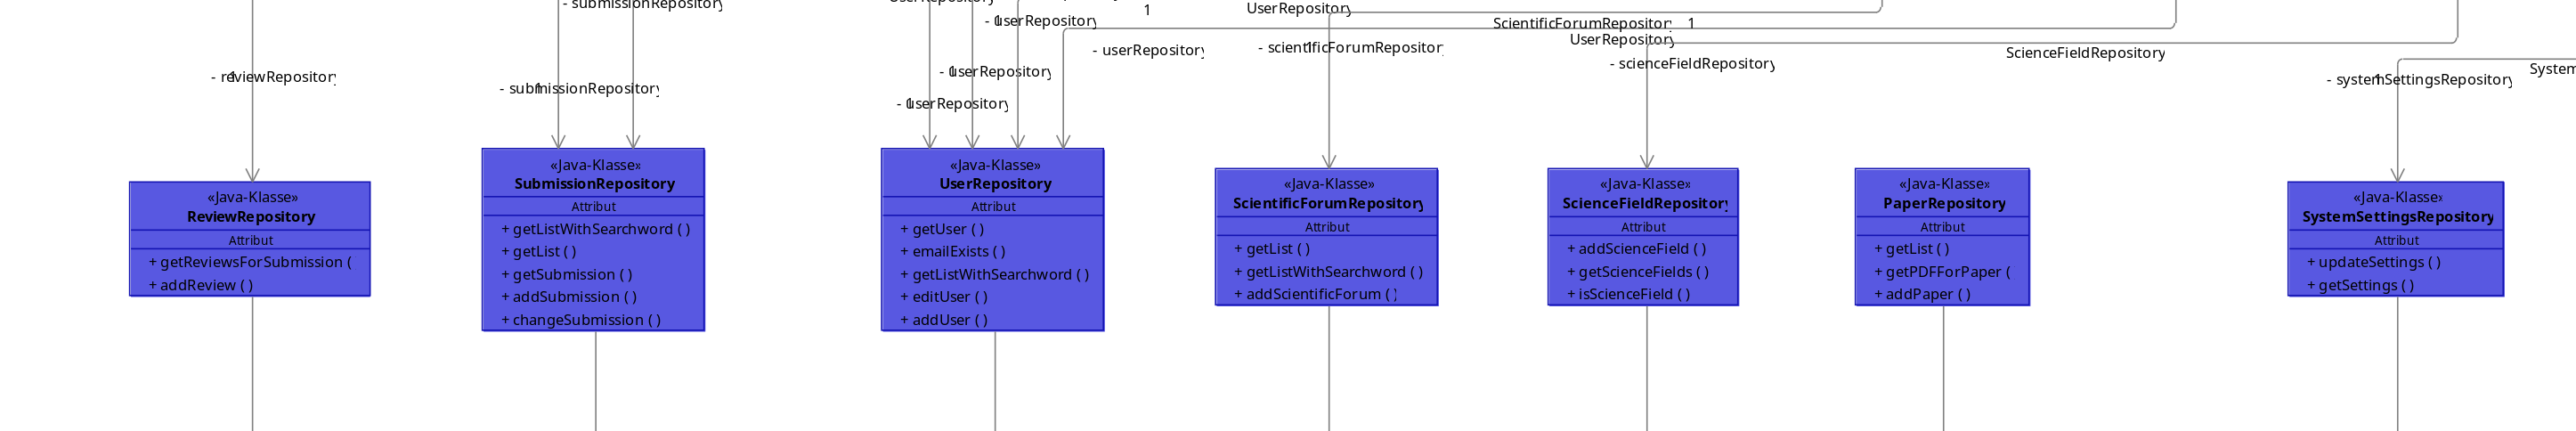
\includegraphics[width=0.9\linewidth]{graphics/persistence_repository}
\end{figure}

\classtable{
    \classentry{PaperRepository}{This repository can get the list of papers for a submission or add new ones.}

    \classentry{ReviewRepository}{This repository can get the reviews for a certain submission and add new ones.}

    \classentry{ScienceFieldRepository}{This repository can get or add new fields of science from/to the database.}

    \classentry{ScientificForumRepository}{This repository can get a list of journals and conferences or add new ones.}

    \classentry{SubmissionRepository}{This repository allows CRUD operations on submissions.}

    \classentry{SystemSettingsRepository}{This repository can read or update the system settings.}

    \classentry{UserRepository}{This repository allows CRUD operations on users.}

    \classentry{ReviewedByRepository}{This respository allows to get and change information about the relationship of a submission and a reviewer.}
}

\subsubsection{de.lases.persistence.util}

\begin{figure}[H]
	\centering
	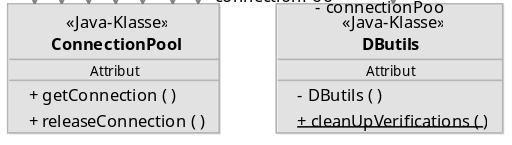
\includegraphics[height=2cm]{graphics/persistence_util}
\end{figure}

\classtable{
    \classentry{ConnectionPool}{Provides and manages connections to the database.}

    \classentry{DButils}{Provides functions for general database services.}

    \classentry{EmailSender}{Talks to the SMTP server.}

    \classentry{ConfigReader}{Reads the global configuration file from the disk.}
}

\subsubsection{de.lases.persistence.exception}

\begin{figure}[H]
	\centering
	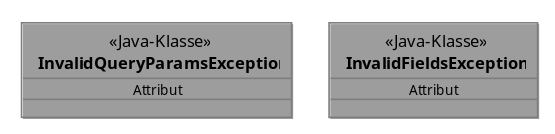
\includegraphics[height=2cm]{graphics/persistence_exception}
\end{figure}

\classtable{
    \classentry{InvalidFieldsException}{Hints at an invalid field in a dto given to the persistence layer.}
    \classentry{InvalidQueryParamsException}{Hints at invalid field in the ResulstListParameters object given to the persistence layer.}
    \classentry{DBConnectionFailedException}{Is thrown when the database connection cannot be established or times out.}
    \classentry{DBConfigurationException}{Is thrown when bad configuration of the database leads to a failure to establish a connection.}
    \classentry{DBQueryFailedException}{Is thrown when a query to the database fails and will probably fail again.}
    \classentry{EmailServiceFailedException}{Fires when the email service used by the application fails unrecoverably.}
    \classentry{ConfigNotReadableException}{Fires when the config file of the application can definitively not be read.}
    \caption{Unchecked Exceptions}
}

\classtable{
	\classentry{EmailAddressExistsException}{Is thrown when the repository tries to save an email-address to the databse that already exists in the database.}
	\classentry{DataNotWrittenException}{Is thrown when the writing of data fails but a retry has a high probability of succeeding, for example when a DataTruncationException occurs.}
	\classentry{DataNotCompleteException}{Is thrown when the reading of data yields an incomplete result but a retry has a high probability of succeeding, for example when a DataTruncation warning occurs.}
	\classentry{NoPermissionException}{Is thrown when a user does not have the correct role to complete a certain operation. This was most likely caused by a race condition where someone lost a role during completion of an operation.}
	\classentry{NotFoundException}{Is thrown when a queried object is not found in the database. In the common case this is caused by a race condition where an object was removed while being selected.}
	\classentry{EmailTransmissionFailed}{Fires whenever the transmission of an email (to a specific list of senders) fails but the email service of this system is intact.}
	\caption{Checked Exceptions}
}

